%!TEX root = main.tex

\section{The Precise Setting: Present-day Visual Querying Systems}\label{sec:precise}
While visual data exploration often reveals 
important anomalies or trends 
in the data~\cite{Heer2012,Morton2014}, 
it is challenging to 
use visualization-at-a-time systems to 
repeatedly choose the right subset of 
data and right attributes to visualize
in order to identify desired insights.
We first motivate
the precise setting using a use-case from
astronomy.

\subsection{Motivating Example: Discovering Patterns in Astronomical Data}
Astronomers from the the Dark Energy Survey (DES) 
are interested in finding 
anomalous time series 
in order to discover 
astrophysical transients, 
i.e., objects whose brightness 
changes dramatically as a function of time, 
such as supernova explosions or quasars~\cite{Drlica-Wagner2017}. 
When trying to find celestial objects 
corresponding to supernovae, 
which have a specific pattern of brightness over time, 
scientists individually inspect the corresponding 
visualizations for each object until 
they find ones that match the pattern. 
With more than 400 million objects in their catalog, 
each having their own set of time series brightness measurement, 
manually exploring so many 
visualizations is not only error-prone, 
but also overwhelming.
The astronomers instead rely on guess-work 
or prior evidence to explore the visualizations,
rather than directly ``searching'' for the patterns
that they care about. 
While a few astronomers do use 
programming tools, such as Python and R,
it is cumbersome to express each new need
via carefully hand-optimized code. 
The astronomy use case highlights a 
common challenge in visual data exploration,
where there are a number of visualizations
for each discovery goal,
and manual exploration is impossible.
There is no systematic way to create, compare, filter,
and operate on large collections of visualizations.

\subsection{Discovering Patterns, Anomalies/Clusters, and Performing Comparisons with \zv}


\par \zv is an example of a visual querying system (VQS) that operates on 
large collections of visualizations.
\zv is built on top of a visual query language
called ZQL, which operates on collections of visualizations, and returns
collections of visualizations,
using primitives such as visualization composition,
sorting, and filtering~\cite{Siddiqui2016}. 
In addition, via user defined functions (also provided as built-ins),
ZQL can compute the distance for a visualization from another---and this
distance can be used as a building block for more complex
operations, such as the first three discovery goals listed
in Table~\ref{fig:table}, i.e., finding a visualization
matching a pattern, detecting an outlier or cluster centers,
or comparing visualizations with each other.
Thus, ZQL operates at a level higher than
languages for specifying visual encodings of
individual visualizations~\cite{Stolte2002,Wilkinson2005}.
ZQL can be used to construct a rich variety of queries,
including the following on a real-estate dataset:
\squishlist
	\item {\em Find Patterns.} Find visualizations of cities whose sales price over time is similar to Manhattan. 
	\item {\em Identify Anomalies.} Find visualizations of cities with an increasing sales price trend, with a simultaneous increasing foreclosure rate trend.
	\item {\em Perform Comparisons.} For New York and Champaign, find visualizations on which they differ the most.
	\item {\em Find Patterns, followed by Clusters.} For cities that are similar
	to New York on sales price trends, find typical trends for foreclosure rates.
\squishend

\par While ZQL is a useful starting point, writing ZQL
queries can be daunting for users who are not comfortable
with programming.
Therefore, we extracted a typical workflow
of visual querying for finding patterns and identifying
outliers and clusters, and made it expressible
via simple interactions---see Figure~\ref{fig:modalities}.
\agp{refer to the figure as this is described.}
The user can input their search pattern via a sketch,
or by inputting a set of points,
and specify a space of visualizations over which to search.
The system returns a ranked list of matching visualizations
for the corresponding ZQL query.
The system also provides typical trends and outliers
for additional context. 
The user can drag-and-drop one of these visualizations
into the sketch panel, starting a search with the corresponding
sketch.
The user can also switch to a tabular interface wherein
they can input ZQL queries.  
Users can also make comparisons between different 
subsets of the data by examining visualizations 
of dynamically created classes in \zv~\cite{Lee2017}.

\begin{figure}[h!]
\centering
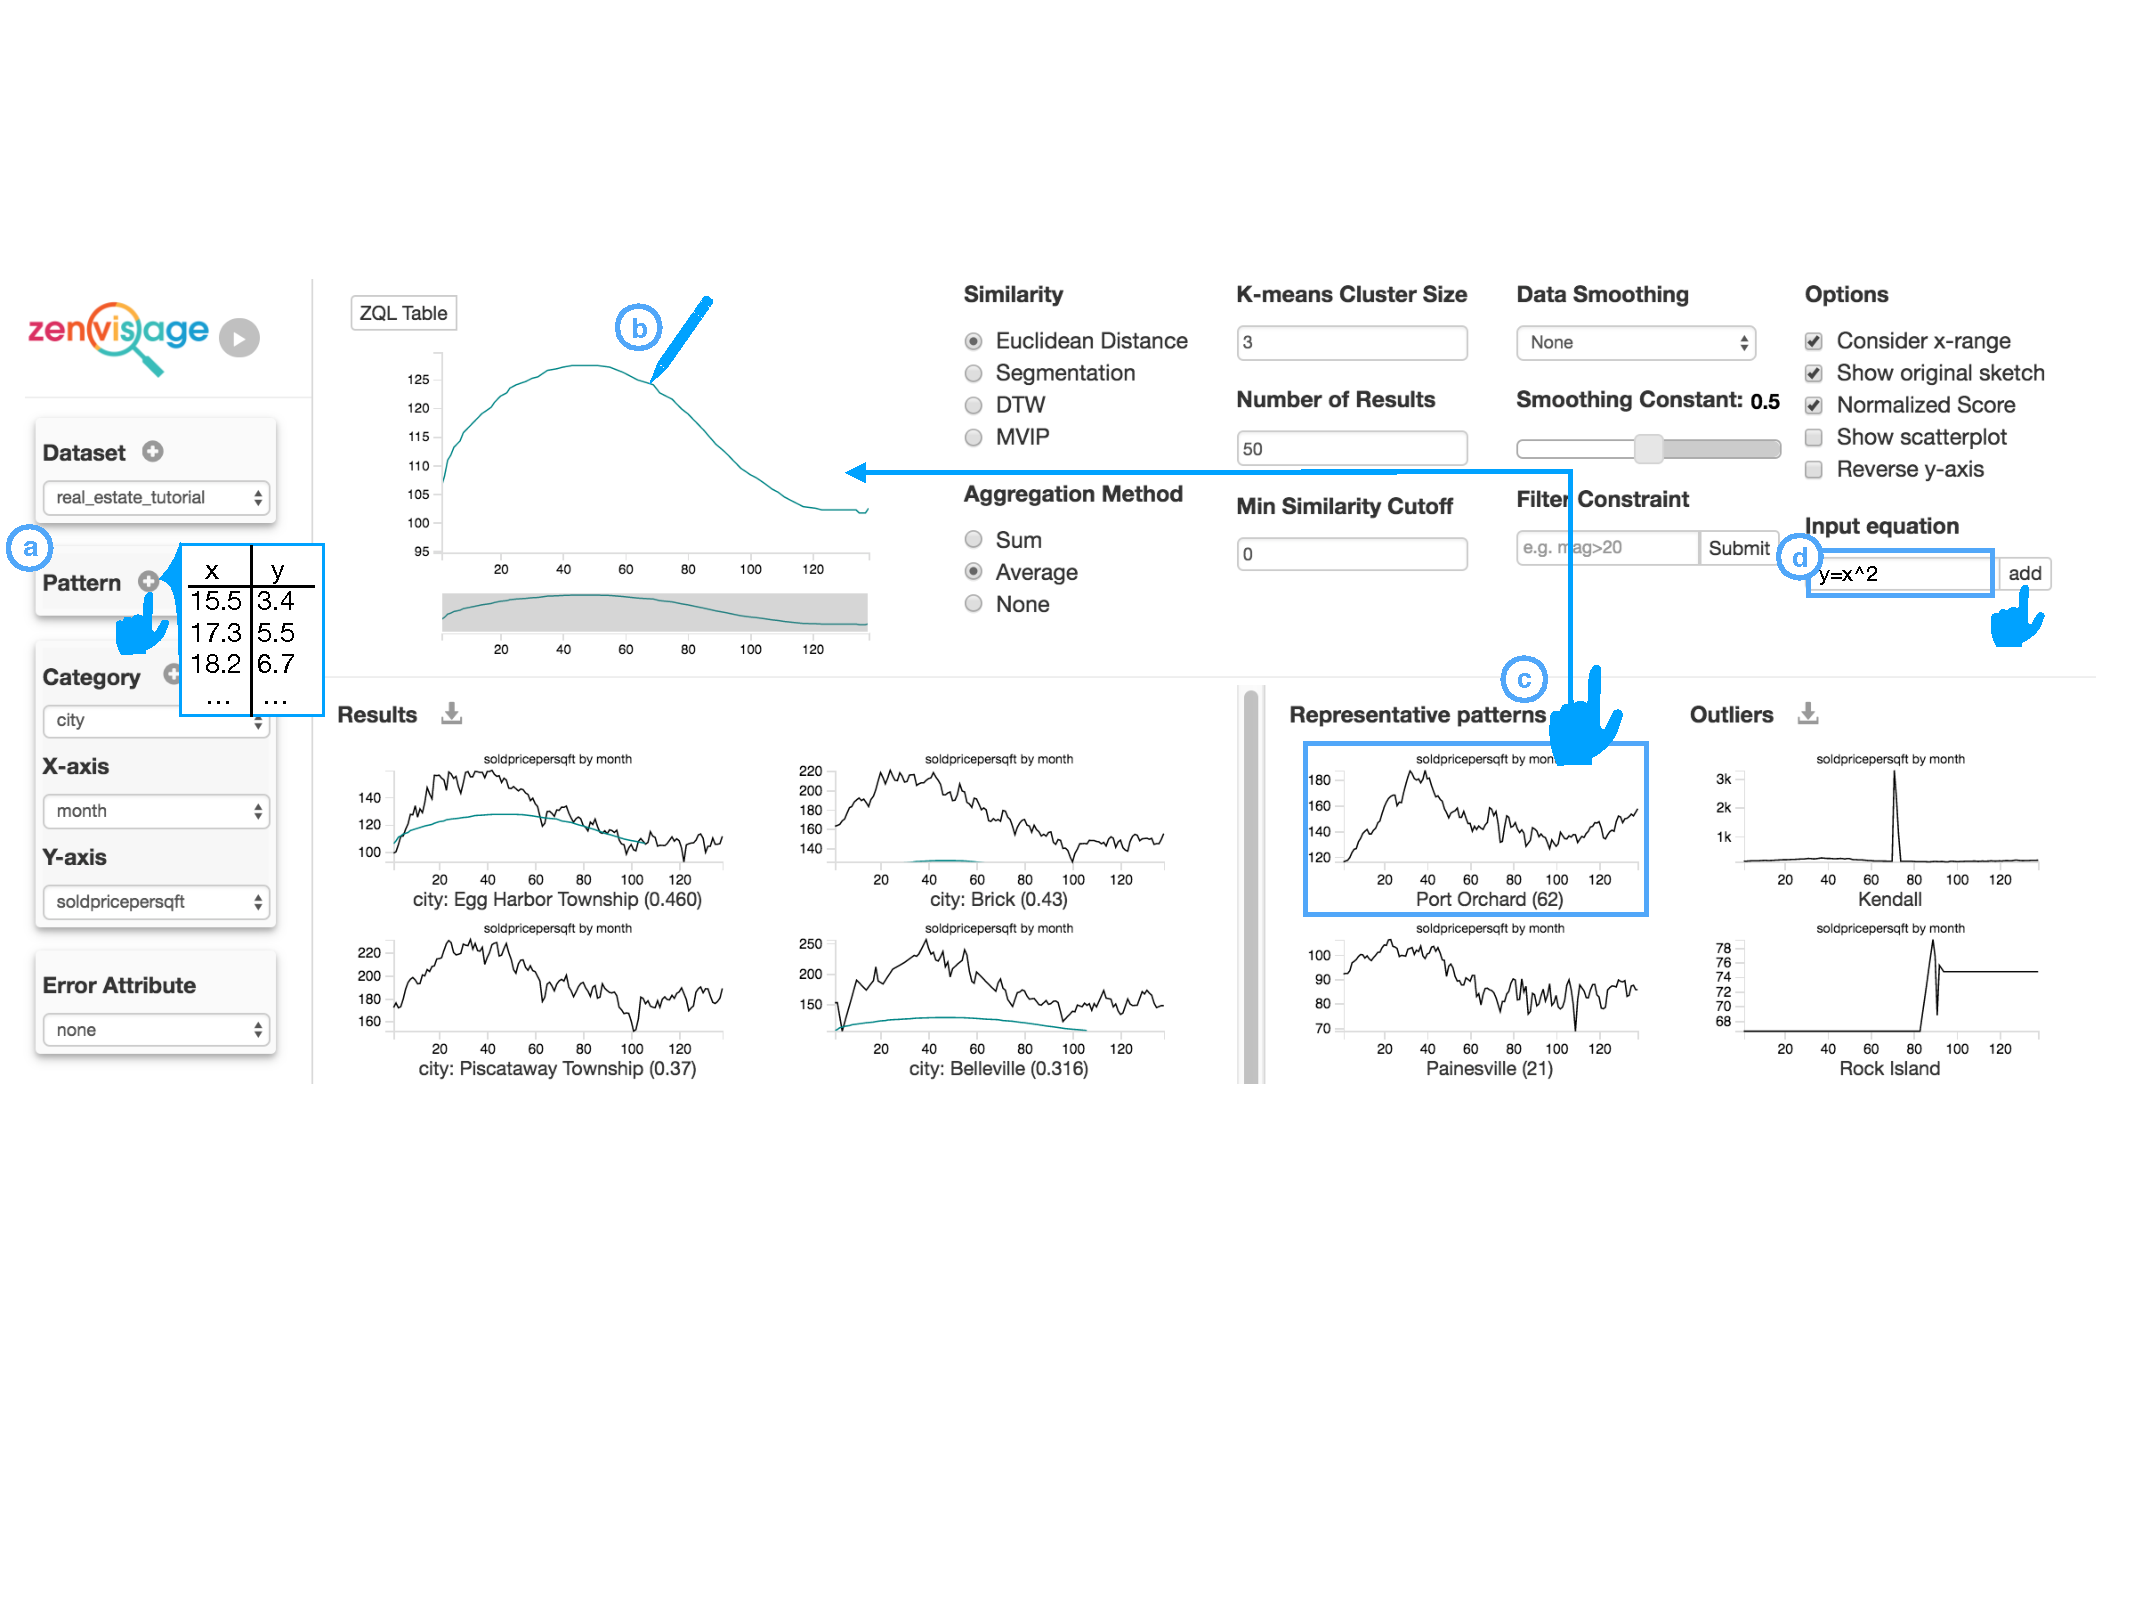
\includegraphics[width=0.8\textwidth]{figures/modalities.pdf}
\caption{\zv offers a variety of querying modalities, including: a) uploading a sample pattern from an external dataset as a query, b) sketching a query pattern, c) dragging-and-dropping an existing pattern from the dataset, and d) inputting an equation as a query, from \cite{Lee2017}.}
\label{fig:modalities}
\end{figure}


\subsection{Other Related Precise Visual Querying Systems}

\agp{For finding patterns: Describe TimeSearcher, Query By Sketch, google correlate, querylines, Correll and Gleicher, Squeries, plus their interactions}

\subsection{Research Challenges within the Precise Setting}

\agp{describe other open questions}
\agp{{\em How do we express the rest of ZQL with intuitive
interactions? How can we support analogous pattern search 
metaphors for other types of visualizations, such as scatterplots
or heatmaps?}}



\subsection{Limitations with the Precise Setting}
\par \zv was developed in collaboration with
scientists from astronomy, genetics, 
and material science via a year-long 
participatory design process~\cite{Lee2017}. 
The findings from that study identifies 
limitations within
the precise setting that need to be addressed
within a full-fledged \vida.


\stitle{The Problem of Interpreting Ambiguous, High-level Queries.}
When users interact with \zv, 
they often translate their ambiguous, 
high-level questions 
into an plan that consists of multiple interactions 
to incrementally address their desired query. 
The expressiveness of such a system 
comes from the multiplicative effect 
of stringing together combinations of 
interaction sequences into a customized workflow. 
Designing features that diversifies potential 
variations expands the space of possible workflows 
that could be constructed during the analysis. 
However, even with many supported interactions, 
there were still vague and complex queries 
that could not be decomposed 
into a multi-step interaction workflow. 
For example, \zv was unable to support 
high-level queries that involved the use of vague 
descriptors for matching to specific data 
characteristics, such as finding patterns that 
are `flat and without noise', or `exhibits irregularities'. 
These scenarios showcase examples of lexical ambiguity, 
where the system can not map the vague term `irregular' or `noisy' 
into the appropriate series of analysis steps 
required to find these patterns. 
In Section~\ref{sec:vague}, we survey the challenges 
in supporting vague and complex queries 
and point to some ongoing research.

\stitle{The Problem of Not Knowing What to Query.}
Another key finding is that 
users often do not start their analysis 
with a specific pattern in mind or a specific comparison to perform. 
For example, within \zv, many users 
first made use of the recommended 
representative trends and outlier visualizations 
as contextual information 
to better understand their data, 
or to query based on these recommended visualizations.
Thus, the recommended visualizations
are often used to form queries in a bottom-up
manner, rather than users coming up with a query
in a top-down, prescriptive manner.
Thus, there is a need for visualization recommendations~\cite{Vartak2017}
that can help users jump-start their exploration.
Recommendations help facilitate a smoother flow
of analysis by closing the gap between the two modalities
of querying and exploration, 
reminiscent of the browsing and searching 
behaviors on the Web~\cite{Olston2003}, thus 
ensuring that user is never stuck or out of 
ideas at any point during the analysis. 
Typically, visualization recommendations help 
accelerate the process of discovering 
interesting aspects of the data by broadening exploration. 
In Section~\ref{sec:minimal}, we argue 
that recommendations should not just focus on 
data discoverability aspect of exploration\agp{what does data discoverability mean?}, but also contribute towards helping users become more aware of the distributions in their data and the context of their analysis.
% % \subsection{Top-down and Bottom-up Querying Modalities}
% % \par Our study also revealed the challenges of coming up with a query in a prescriptive manner. 
% % Need a topic sentence/paragraph
% \par Pirolli and Card's notional model distinguishes between information processing tasks that are \textit{top-down} (from theory to data) and \textit{bottom-up} (from data to theory)~\cite{Pirolli}. In the context of visual querying, users employ top-down approaches by starting with a hypothesis on what patterns to look for and express it through sketching or inputting an equation (Figure~\ref{fig:modalities}b,d). On the other hand, bottom-up approaches originate from the data (or equivalently, the visualization). For example, the user may drag and drop a visualization of interest in the dataset as the input query or upload a visualization from an external dataset (Figure~\ref{fig:modalities}a,c). These two modalities of querying are reminiscent of the browsing and searching behaviors on the Web, which derives from the successful application of foraging theory to Web Search~\cite{Olston2003}.
% \par While the usage of each querying feature may vary from one participant to the next, our interactions with the scientists showed that \emph{bottom-up querying via drag-and-drop was more intuitive and more commonly used than top-down querying methods when the users have no desired patterns in mind}, which is commonly the case for exploratory data analysis. One of the main reason why participants did not find sketching useful was that they often do not start their analysis with a pattern in mind. Later, their intuition about what to query is derived from other visualizations that they see in the PVQS, in which case it made more sense to query using those visualizations as examples directly. Similarly, while functional fitting is a common operation in scientific data analysis, querying by equation is also unpopular, since it is challenging to formulate functional forms in an prescriptive, ad-hoc manner without seeing what the common patterns in the dataset are. 
%  %(e.g. after a filter is applied)  (e.g. find visualizations that are similar to the one in the largest representative clusters). 
% \par As evident from the representative and outliers visualization recommendations in \zv, recommendations facilitate a smoother flow of analysis by closing the loop between the two modalities of querying and exploration, thus ensuring that user is never stuck or out of ideas at any point during the analysis. Typically, visualization recommendation systems seeks to accelerate the process of discovering interesting aspects of the data by broadening exploration. In Section~\ref{sec:understanding}, we advocate recommendation systems should not only focus on data discoverability aspect of exploration, but also contribute towards helping users become more aware of the distributions in their data and the context of their analysis.


%While this could be expressed through user-defined functions in the underlying querying language ZQL, the learning curve and engineering cost is high. %Our previous example of queries that could not be expressed in the \zv interface showcases one example of  %\dor{Not sure if its worthwhile to include a couple sentences about Tarique's regex/NLP work here. e.g. the `up and then down' example}. 
%Participants in our \zv design study often created unexpected workflows that chained together analysis steps consisting of multiple interactions and controls. For example, geneticists in our study repeatedly explored representative trends to gain an overall sense of the typical profiles that exist in their dataset and queried mainly through drag-and-drop of these representative trends. Variations to their main workflow also include changing cluster sizes and display control settings to offer them different perspectives on the dataset. 